\documentclass[11pt,a4paper]{article}
\usepackage[T1]{fontenc}
\usepackage[utf8]{inputenc}
\usepackage[margin=19mm,headheight=14pt]{geometry}
\usepackage{lmodern,amsmath,amssymb,booktabs,xcolor,listings,enumitem,fancyhdr,graphicx}
\usepackage{placeins}
\usepackage[colorlinks=true,linkcolor=blue!50!black,urlcolor=blue!50!black]{hyperref}
\setlength{\parindent}{0pt}
\setlength{\parskip}{5pt}
\setlist[itemize]{leftmargin=*,topsep=3pt,itemsep=2pt,parsep=0pt}
\setlist[enumerate]{leftmargin=*,topsep=3pt,itemsep=2pt,parsep=0pt}
\pagestyle{fancy}
\fancyhf{}
\fancyhead[L]{Bayesian neural networks}
\fancyhead[R]{Teacher's guide}
\fancyfoot[C]{\thepage}
\definecolor{codebg}{RGB}{246,247,249}
\lstset{language=Python,basicstyle=\ttfamily\footnotesize,
  keywordstyle=\color{blue!55!black},commentstyle=\color{black!60},
  stringstyle=\color{green!35!black},backgroundcolor=\color{codebg},
  frame=single,rulecolor=\color{black!15},framesep=5pt,
  showstringspaces=false,keepspaces=true,columns=fullflexible,
  breaklines=true,aboveskip=6pt,belowskip=6pt}
\newcommand{\E}{\mathbb E}
\newcommand{\Var}{\operatorname{Var}}
\newcommand{\KL}{\operatorname{KL}}
\newcommand{\Normal}{\mathcal N}
\newcommand{\R}{\mathbb R}
\newcommand{\MI}{\operatorname{I}}
\newcommand{\dd}{\,d}
% Normal weight throughout prose, titles, and headings.
\makeatletter
\renewcommand\section{\@startsection{section}{1}{\z@}%
  {-3.5ex \@plus -1ex \@minus -.2ex}%
  {2.3ex \@plus .2ex}{\normalfont\Large}}
\renewcommand\subsection{\@startsection{subsection}{2}{\z@}%
  {-3.25ex \@plus -1ex \@minus -.2ex}%
  {1.5ex \@plus .2ex}{\normalfont\large}}
\renewcommand\subsubsection{\@startsection{subsubsection}{3}{\z@}%
  {-3.25ex \@plus -1ex \@minus -.2ex}%
  {1.5ex \@plus .2ex}{\normalfont\normalsize}}
\makeatother
\begin{document}
\begin{center}
 {\LARGE Bayesian neural networks: predictions, uncertainty, and active learning}\\[6pt]
 {\large Teacher's guide and worked solutions}\\[3pt]
 Bayesian machine learning \textbar\ Skoltech
\end{center}

A neural classifier gives a probability vector at an input. A Bayesian model
also represents uncertainty over its parameters and averages predictions over
that uncertainty. This seminar uses Monte Carlo dropout as a practical
approximation, separates predictive entropy from model disagreement, and
uses disagreement to decide which labels to request next.

Tasks 1--3 form a 90-minute core on a one-dimensional example. Task 4 is a
separate 45--60-minute GPU practical on MNIST active learning. The image model,
training loops, and plotting are supplied. Students implement the calculations
that connect model draws, probabilities, uncertainty scores, and acquisition.
The companion student and solutions notebooks share their lesson order;
this guide provides derivations, worked answers, hints, and interpretation.

The central distinction is between a probability estimated accurately under
an approximate model and a probability that is accurate for the real data.
More dropout draws reduce Monte Carlo error for the fitted approximation.
They do not repair its posterior approximation, training error, or a mismatch
between the model and the data-generating process.

\section{Teaching plan}
\subsection{The 90-minute core}
The clock includes exercise time. Use the supplied optimizer and figures
without explaining every line of their implementation. Keep the connection
from posterior averaging to the label-acquisition decision visible throughout.
\begin{center}
\begin{tabular}{@{}p{15mm}p{48mm}p{94mm}@{}}
\toprule
Clock & Topic & Student activity and intended result \\
\midrule
0--10 & Posterior and toy data & Identify the two sources of prediction
randomness and inspect observed intervals and the gap. \\
10--20 & MC dropout & Distinguish stochastic model draws, deterministic evaluation,
and coherent function curves. \\
20--35 & Task 1: predictive probabilities & Transform logits to probabilities
before averaging; verify shapes and model-mode restoration. \\
35--45 & Entropy and disagreement & Work through two predictive distributions
with the same mean and different disagreement. \\
45--60 & Task 2: uncertainty decomposition & Calculate categorical entropy,
expected conditional entropy, and mutual information. \\
60--70 & BALD and the oracle & Derive the information score and identify which
labels the acquisition code may access. \\
70--83 & Task 3: active acquisition & Choose unique pool indices; compare
label budgets and controlled acquisition runs. \\
83--90 & Interpretation & Explain the finite Monte Carlo limit and distinguish
an illustrative result from a general acquisition guarantee. \\
\bottomrule
\end{tabular}
\end{center}

Before class, run the complete solutions notebook on the actual classroom
machine. The core uses PyTorch, NumPy, Matplotlib, and notebook display tools;
its data are generated locally and it runs on CPU. The image extension also
needs compatible TorchVision, CUDA, and a cached MNIST dataset. Keep the
executed solution figures available if classroom training takes longer than
expected. Students need Bayes' rule, categorical probabilities, logarithms,
expectations, and basic PyTorch tensor operations.

Protect the active-learning endpoint. Start the entropy implementation by
minute 45 and discuss the oracle by minute 60. If a function is unfinished,
explain its missing mathematical operation and continue with the working
solution. Shorten optimizer mechanics and extra architecture experiments
before removing the uncertainty decomposition or the budget comparison.

For a 60-minute version, allocate 0--8 minutes to posterior prediction and
the toy geometry, 8--20 to Task 1, 20--35 to Task 2, 35--47 to BALD and Task 3,
47--57 to the controlled comparison, and 57--60 to closing questions. Show
already executed training results. Keep the nonlinear averaging step, the
entropy-versus-disagreement example, and the no-label-peeking acquisition rule.

\subsection{The separate GPU practical}
Allow 45--60 additional minutes for Task 4. Allocate approximately 10 minutes
to the multiclass model and data split, 10--15 to minibatch MC prediction and
its checks, 15--20 to the supplied acquisition experiment, and 10--15 to
learning curves, acquired images, and paired comparisons. Run the complete
experiment before class. This teaching allocation is not a hardware-independent
promise about training runtime.

\subsection{Board notation}
\begin{center}
\begin{tabular}{@{}p{36mm}p{121mm}@{}}
\toprule
Object & Meaning \\
\midrule
$w$, $p(w\mid\mathcal D)$ & Neural-network weights and their Bayesian posterior. \\
$q_\phi(w)$ & Approximation used to generate stochastic model draws. \\
$p_c(x,w)$ & Conditional class probability for class $c$ at fixed weights. \\
$\bar p_c(x)$ & Probability averaged over the fitted weight approximation. \\
$\Pi\in\R^{T\times N\times C}$ & $T$ model draws, $N$ inputs, and $C$ classes;
the class probabilities sum to one along the last axis. \\
$H_{\rm pred}$, $H_{\rm cond}$ & Entropy of the mean probability vector and mean
conditional entropy across model draws. \\
$\MI_q(Y;W\mid x)$ & Model-relative disagreement, $H_{\rm pred}-H_{\rm cond}$. \\
$\mathcal L$, $\mathcal U$ & Labeled training set and remaining unlabeled pool. \\
\bottomrule
\end{tabular}
\end{center}
All entropies in the notebooks use natural logarithms, so their unit is nats.
Do not compare their numerical values with bit entropies without conversion.

\section{Purpose and practical limitations: teacher background}
Use one short motivation in the timed introduction. The full discussion is
preparation material and does not add another block to the 90-minute core.
When labels are costly and unlabeled inputs are plentiful, active learning
turns uncertainty into a proposed annotation decision. A useful experiment
asks whether the chosen rule achieves a specified metric with fewer queried
labels under an explicit budget and comparison protocol.

Gal, Islam, and Ghahramani demonstrate a dropout-based image active-learning
framework on MNIST and an ISIC2016 lesion-image dataset~\cite{gal2017}.
These published examples motivate uncertainty-aware label selection. The
seminar's compact MNIST experiment is a controlled teaching study, not a
reproduction of their architecture, optimization, or results.

High predictive entropy can reflect disagreement among models or ambiguity
within each model. BALD targets the former under its fitted distribution.
Neither score guarantees detection of out-of-distribution inputs, calibration,
or improved accuracy after a particular query. A model can confidently agree
on a wrong extrapolation. An informative label can also be atypical of the
future test population. Check the evaluation distribution, label quality,
class composition, and acquisition cost before interpreting a score as value.

Increasing MC samples, acquiring new labels, and improving optimization act
on different uncertainties. The first improves numerical integration under
one fitted approximation. The second changes the available training
information. The third changes how the approximation is fitted. Keep these
operations separate when explaining the observed curves.

\section{Bayesian neural-network prediction}
\subsection{A discriminative model conditions on its inputs}
Let $\mathcal D=\{(x_i,y_i)\}_{i=1}^n$. For a neural network with logits
$a_w(x)\in\R^C$, define
\[
 p(y=c\mid x,w)=\operatorname{softmax}(a_w(x))_c.
\]
For two classes, a single logit $a_w(x)$ equivalently gives
$p(y=1\mid x,w)=\sigma(a_w(x))$, with
$\sigma(a)=1/(1+e^{-a})$. Conditional independence of labels gives
\[
 p(\mathcal D\mid w)=\prod_{i=1}^n p(y_i\mid x_i,w).
\]
We condition on the inputs. Neither maximum likelihood nor this posterior
calculation requires assuming that inputs are uniformly distributed.
A prior over weights yields
\[
 p(w\mid\mathcal D)=\frac{p(\mathcal D\mid w)p(w)}{p(\mathcal D)},
 \qquad p(\mathcal D)=\int p(\mathcal D\mid w)p(w)\dd w.
\]
The posterior can have many coupled, non-Gaussian directions. Its integrals
are generally unavailable in closed form even when the network evaluates
quickly at a specified weight vector.

\subsection{Average probabilities after the nonlinear network}
The posterior predictive distribution is
\[
 p(y=c\mid x,\mathcal D)=\int p(y=c\mid x,w)p(w\mid\mathcal D)\dd w.
\]
Approximate the posterior by $q_\phi$ and draw $w_t\sim q_\phi$ independently:
\[
 \bar p_c(x)=\E_{q_\phi}[p(y=c\mid x,W)],\qquad
 \widehat p_c(x)=\frac1T\sum_{t=1}^T p(y=c\mid x,w_t).
\]
For a fixed fitted approximation, this sample mean is unbiased for $\bar p_c$
and consistent as $T$ grows. The Bayesian posterior predictive may still
differ from $\bar p_c$ because $q_\phi$ is approximate.

The sigmoid, softmax, and neural network are nonlinear. In general
\[
 \E_q[\sigma(a_W(x))]\ne\sigma(\E_q[a_W(x)]).
\]
For logits $-4$ and $0$ with equal weights, the mean class-1 probability is
approximately $0.2590$; applying the sigmoid to their mean logit gives
$\sigma(-2)\simeq0.1192$. Averaging hard class decisions discards conditional
probability information as well. A deterministic dropout-off evaluation is
another prediction rule, not generally the MC predictive mean.

There are two levels of randomness: first draw a model $W$, then draw the
label $Y$ from that model's categorical probabilities. Conditional model
probabilities can vary across weight draws even when no label is sampled.
For a fixed input, the standard error of their numerical mean is approximately
$s_p/\sqrt T$. Their spread $s_p$ and this standard error answer different
questions. Increasing $T$ shrinks integration error; it does not concentrate
the fitted $q_\phi$ around one network.

\section{MC dropout and its approximation assumptions}
\subsection{What changes between training and prediction}
Dropout multiplies selected activations by a random mask. With drop probability
$r$, inverted dropout uses mask entries $M_j=B_j/(1-r)$ with
$B_j\sim\operatorname{Bernoulli}(1-r)$. Thus $\E M_j=1$, while each mask
defines a different subnetwork. The trained numerical weights remain fixed
during MC prediction; the masks supply the model draws.

Gal and Ghahramani connect dropout training with an approximate variational
Bayesian construction~\cite{gal2016}. This motivates stochastic prediction
with dropout active. It does not make arbitrary dropout settings, priors,
and regularizers an exact posterior inference procedure. A Bayesian
interpretation requires a specified likelihood and prior, a matching
approximating family, and attention to regularization and loss scaling.

In a generic variational formulation,
\[
 \log p(\mathcal D)=\operatorname{ELBO}(q)
              +\KL(q(w)\Vert p(w\mid\mathcal D)),
\]
where
\[
 \operatorname{ELBO}(q)=\E_q[\log p(\mathcal D\mid W)]
                         -\KL(q(w)\Vert p(w)).
\]
A dropout training objective uses stochastic likelihood evaluations and a
regularization surrogate related to the prior term under the approximation's
assumptions. The seminar uses regularized dropout as a practical posterior
approximation. It does not claim an exact KL computation for a Bernoulli
point-mass weight distribution against a continuous Gaussian prior.

Changing dropout probability, architecture, or the regularization strength
changes the fitted approximation. More dropout does not guarantee better
uncertainty, and a bigger predictive spread need not imply better calibration.
Retrain after changing such settings; repeated prediction alone cannot fit
new parameters.

With a mean-loss objective, holding the L2 coefficient fixed while the labeled
set grows changes its equivalent strength in the summed objective. A fixed
Bayesian prior interpretation would need consistent likelihood and regularizer
scaling. The controlled acquisition experiments hold the announced training
policy equal across strategies; they are not an exact sequential posterior
update under a calibrated prior.

\subsection{A model draw must be consistent for a function plot}
To plot $x\mapsto p(y=1\mid x,w_t)$ as one random function, use the same
model realization at every plotted input. Sample the masks once for that
draw and reuse them across the grid. If the grid is split into chunks, keep
the masks fixed across chunks too. Then resample masks for the next function.

Ordinary dropout often draws separate masks for different rows of one batch.
This gives appropriate marginal stochastic predictions at each input, but
joining those rows does not display one sampled function. Independently
resampled masks per input can turn an otherwise smooth curve into artificial
point-to-point noise. The core uses shared realizations for its function plots.

Pointwise entropy and MI require the marginal model distribution at each
input; they do not require coupling different inputs to the same model draw.
The image practical uses independent per-example masks for these marginal
scores. It consequently does not estimate joint information for a batch of
images.

\subsection{Prediction modes and state restoration}
Use gradient-free inference and restore the model's original mode after
sampling. Merely calling \texttt{model.train()} can activate unrelated training
behavior. In particular, batch-normalization layers can update their running
statistics. The supplied helpers separate dropout activation from other
training state and restore all relevant flags afterward. The core's shared
mask mechanism and the CNN's ordinary dropout mechanism have different
purposes; apply the appropriate helper to each.

\section{The requested one-dimensional example}
The geometry comes from the first example of the supplied 2025 uncertainty
seminar. Preserve its four intervals and 30 points per interval:
\begin{center}
\begin{tabular}{@{}lll@{}}
\toprule
Class & Intervals & Observations \\
\midrule
0 & $[-5,-3]$ and $[1,2.5]$ & $30+30$ \\
1 & $[-3,-2]$ and $[2.5,5]$ & $30+30$ \\
\bottomrule
\end{tabular}
\end{center}
There are 120 rows. Inclusive interval endpoints put two observations with
opposite labels at $x=-3$ and at $x=2.5$. These are deliberate consequences
of retaining the original construction, not a reason to silently drop rows.
The interval $(-2,1)$ contains no observations.

For evaluation, the notebook separately specifies a population: choose one of
the intervals uniformly, sample $x$ uniformly inside it, and use that
interval's class. The deterministic 120-point training grid is not itself
a random sample from that population. Shared endpoints have population
probability zero. The population has no mass in the gap, so a ground-truth
conditional label probability there is not identified by this definition.
The network still produces a conditional prediction at such an input.

\begin{figure}[htbp]
\centering
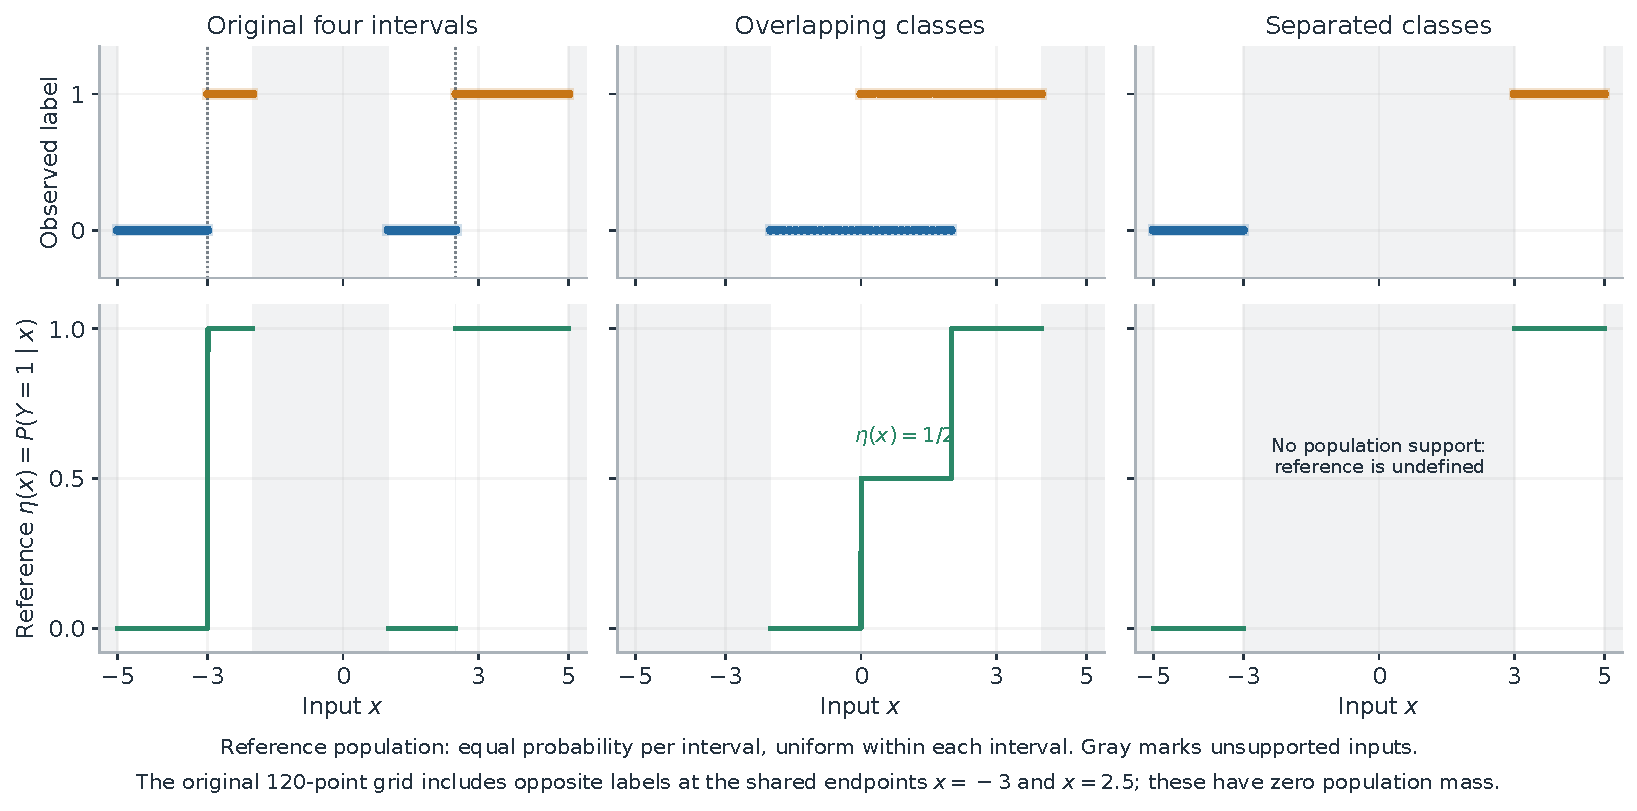
\includegraphics[width=\linewidth]{assets/interval_geometry.pdf}
\caption{The retained four-interval design and two optional variants. Reference
probabilities belong to an explicitly specified mixture-of-intervals
population. Gray indicates inputs outside that population's support; the
reference conditional probability is left undefined there.}
\end{figure}

Inspect predictions near observed interiors, the shared boundaries, the gap,
and beyond the observed range. Observed conflicting labels at the shared endpoints and missing observations
in the gap are different properties of the training design.
The fitted uncertainty curves are evidence about this network approximation;
they need not respond perfectly to either property. In particular, an empty
gap does not mathematically force MC-dropout disagreement to be high.

\FloatBarrier
\section{Task 1: posterior predictive probabilities}
\subsection{What students should do}
Complete the function
\begin{lstlisting}
mc_probabilities(model, inputs, n_draws=200)
\end{lstlisting}
Return a tensor with shape $(T,N,C)$: draw, input, class. Use the supplied
\texttt{sampled\_model} context separately for every draw. It enables the
appropriate stochastic modules, holds each shared feature mask fixed across
the entire input batch, disables gradients, and restores all previous module
modes and MC state in a finally block. Apply softmax along the class axis
before stacking draws. Do not average inside this function; later cells need
the individual probability vectors.

\subsection{Worked implementation}
\begin{lstlisting}
def mc_probabilities(model, inputs, n_draws=200):
    if n_draws < 1 or len(inputs) == 0:
        raise ValueError("Need at least one draw and one input")
    draws = []
    for _ in range(n_draws):
        with sampled_model(model):
            draws.append(model(inputs).softmax(dim=-1))
    return torch.stack(draws, dim=0)
\end{lstlisting}
For a class-1 mean, use \texttt{draws.mean(dim=0)[:, 1]}. Calling softmax after
averaging logits evaluates a different distribution. Returning the mean
alone would also discard the information needed for the MI calculation.

\subsection{The supplied original-architecture experiment}
The retained MLP has widths $1\to10\to50\to20\to1$, sigmoid hidden
activations, and dropout probability 0.2 before the sigmoid after the
50-unit layer. For a scalar final logit $a$, the wrapper returns two logits
$(-a/2,a/2)$. This preserves the binary model because
\[
 \operatorname{softmax}(-a/2,a/2)_1=\frac{e^{a/2}}{e^{-a/2}+e^{a/2}}
 =\sigma(a).
\]
Cross entropy on these centered logits is the corresponding stable binary
logit loss. Preserve the fixed transformation from the original input range
$[-5,5]$ to $[0,1]$; do not refit normalization from each acquired subset.
This uses a known input range, not hidden candidate labels.

The supplied reference fit uses 4,000 full-batch Adam steps, learning rate
0.01, weight decay $10^{-4}$, and a OneCycle schedule with maximum learning
rate 0.1. Training is supplied so that the exercise focuses on prediction.
The main prediction experiment uses 200 model draws. It shows coherent
sampled probability functions, their average, and deterministic dropout-off
evaluation. These are different objects even when their curves happen to
lie close together.

The pointwise 5--95\% range is an empirical range of model probabilities
across dropout draws. It is not a label interval, an interval for the Monte
Carlo mean, or a simultaneous coverage band for the whole function. The
probability mean's MC standard error is calculated separately. Neither range
is a guarantee of calibrated Bayesian posterior coverage.

\subsection{Checks, hints, and interpretation}
Check the full $(T,N,C)$ shape, normalization along classes, finite values,
absence of gradient history, and restoration of model state. A zero-dropout
network gives the same probabilities in every draw. A stochastic network
should vary across independent draws. Repeated inputs within one shared-mask
draw must agree; this distinguishes a coherent model function from independent
per-row perturbations.

If a student averages logits, use the two-logit numerical example from the
board. If all stochastic curves coincide, inspect whether masks were refreshed
between draws. If curves are noisy from one input to the next, inspect whether
one mask was reused within the draw. A graph of attractive curves alone does
not verify the posterior approximation.

A suitable interpretation states that probabilities are averaged after the
nonlinear model, the dropout-off curve need not equal that mean, and more MC
draws improve numerical precision rather than refitting the network.

\begin{figure}[htbp]
\centering
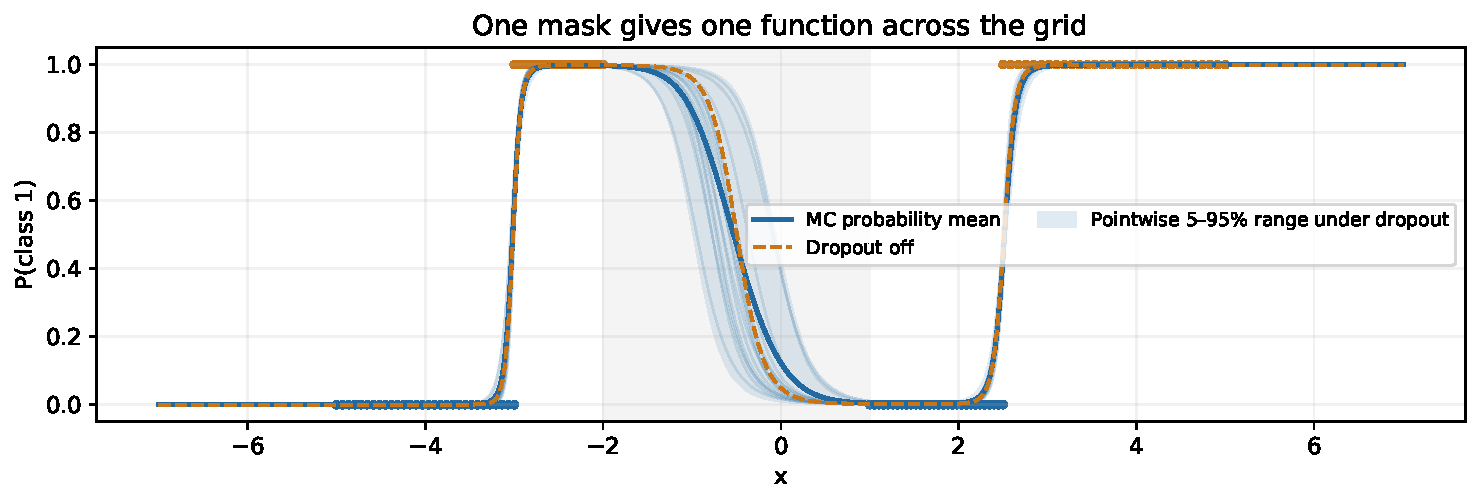
\includegraphics[width=\linewidth]{assets/toy_mc_predictions.pdf}
\caption{The reused interval example, with coherent dropout functions,
their mean and their pointwise probability range. The dashed evaluation
curve is a different calculation from averaging stochastic probabilities.}
\end{figure}

In the executed reference fit, the grid point $x\simeq-1.008$ has class-1
mean probability 0.8684, component-probability standard deviation 0.1516,
and MC standard error 0.01072 from 200 draws. The last is approximately the
second divided by $\sqrt{200}$. At $x\simeq5.992$, outside the training
range, the model is very confident: mean probability 0.99975. This is a
useful counterexample to a claim that missing observations automatically
produce uncertain extrapolation.

\section{Categorical uncertainty and mutual information}
\subsection{Entropy has a specified random variable}
For a categorical probability vector $p\in[0,1]^C$,
\[
 H(p)=-\sum_{c=1}^C p_c\log p_c,\qquad 0\log0:=0.
\]
It lies between zero and $\log C$. A point-mass label distribution has entropy
zero, while the uniform distribution maximizes it. A probability is a number;
entropy is a property of an entire categorical distribution.

For the model mixture at input $x$, define
\begin{align*}
 H_{\rm pred}(x)&=H(\E_q[p(\cdot\mid x,W)]),\\
 H_{\rm cond}(x)&=\E_q[H(p(\cdot\mid x,W))],\\
 \MI_q(Y;W\mid x)&=H_{\rm pred}(x)-H_{\rm cond}(x).
\end{align*}
The first is total label uncertainty under the fitted mixture. The second
is uncertainty remaining when a model draw is known. The difference measures
how much learning a label can distinguish current model draws.

These are often called total, aleatoric, and epistemic uncertainty. In the
seminar they are model-relative quantities. The conditional term need not
identify the true irreducible noise of nature: misspecification, underfitting,
and posterior approximation affect it. Agreement among confidently wrong
models gives small MI even when their predictions fail on new inputs.

\subsection{Same predictive mean, different uncertainty}
Consider two equally weighted model draws for binary classification:
\begin{center}
\begin{tabular}{@{}lccc@{}}
\toprule
Draw probabilities & $H_{\rm pred}$ & $H_{\rm cond}$ & MI \\
\midrule
Both $(0.5,0.5)$ & $\log2$ & $\log2$ & 0 \\
$(1,0)$ and $(0,1)$ & $\log2$ & 0 & $\log2$ \\
Both $(0.99,0.01)$ & 0.0560 & 0.0560 & 0 \\
\bottomrule
\end{tabular}
\end{center}
The first two cases have the same predictive probability $(0.5,0.5)$ and
entropy $\log2\simeq0.6931$. In the first, both models predict an ambiguous
label. In the second, each predicts confidently, but they disagree about the
label. Predictive entropy alone cannot distinguish these explanations.


\begin{figure}[htbp]
\centering
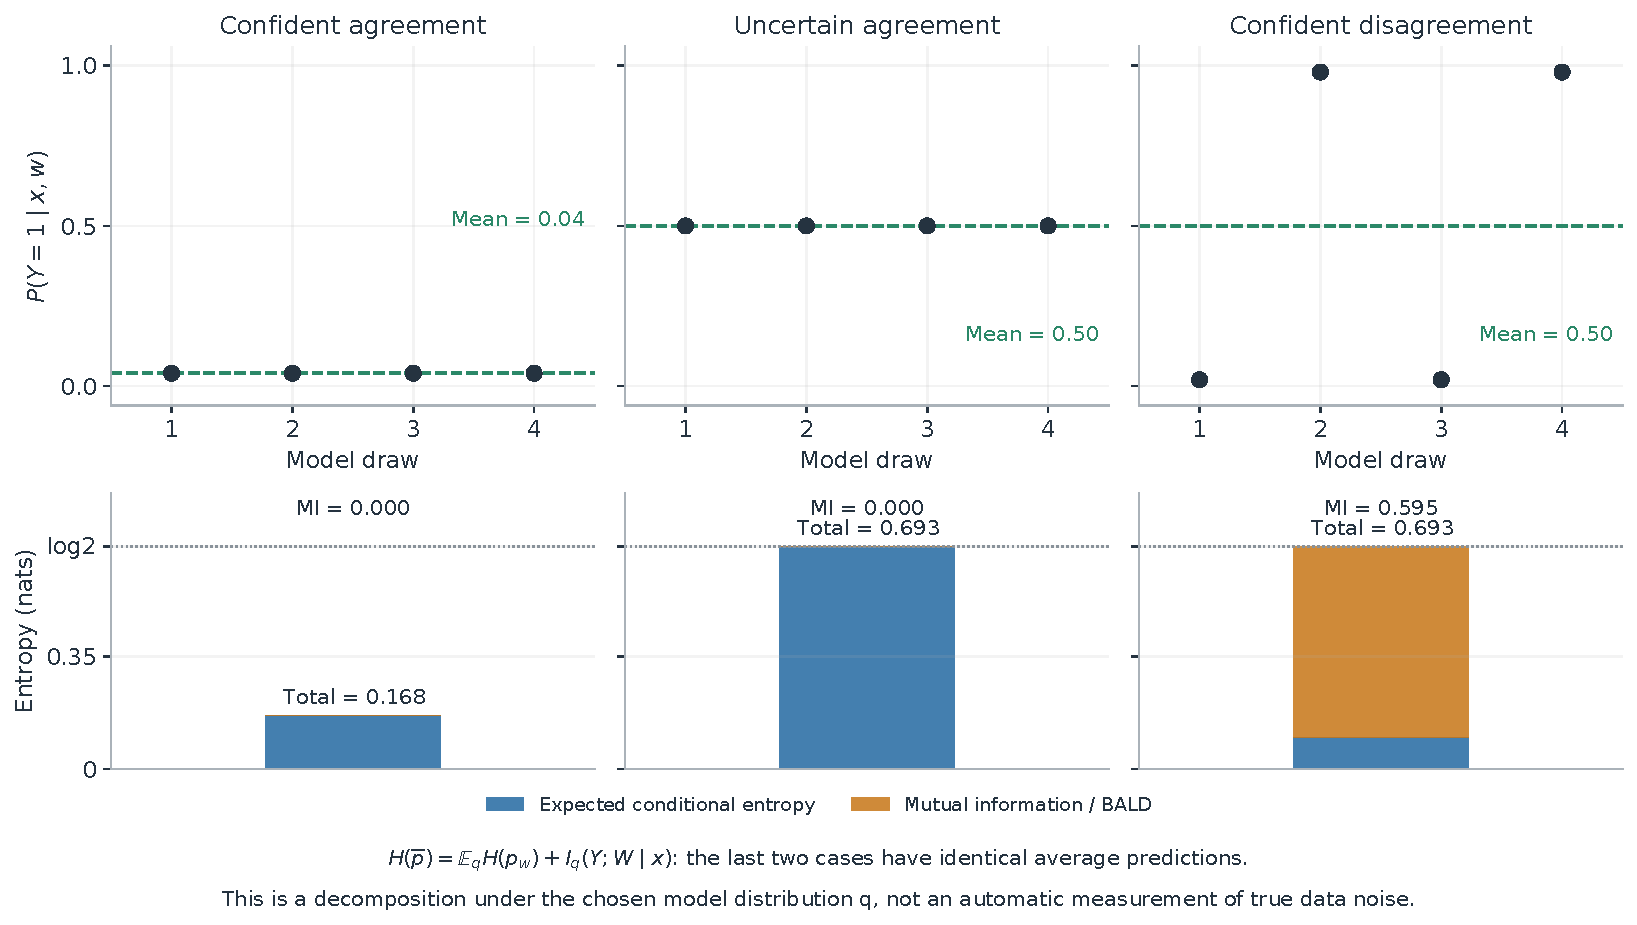
\includegraphics[width=\linewidth]{assets/uncertainty_decomposition.pdf}
\caption{Agreement and disagreement can have different uncertainty
interpretations. A mixture of confident, conflicting predictions can have
the same mean as predictions that are individually ambiguous. The displayed
decomposition is under the chosen model distribution.}
\end{figure}
\subsection{Finite Monte Carlo calculations and bias}
Given $\Pi_{tic}=p(y=c\mid x_i,w_t)$, calculate
\begin{align*}
 \widehat p_{ic}&=\frac1T\sum_t\Pi_{tic},\\
 \widehat H_{{\rm pred},i}&=H(\widehat p_i),\\
 \widehat H_{{\rm cond},i}&=\frac1T\sum_t H(\Pi_{ti}),\\
 \widehat I_i&=\widehat H_{{\rm pred},i}-\widehat H_{{\rm cond},i}.
\end{align*}
Sum over classes inside entropy; average model draws along the first axis.
Retain one score per input. Entropy concavity implies $\widehat I_i\geq0$
in exact arithmetic. A substantially negative value indicates a shape,
normalization, or formula error. Tiny negative roundoff can be handled at the
reporting boundary; clipping must not hide an incorrect implementation.

For iid draws, $\widehat p$ is unbiased and the mean conditional entropy is
unbiased for its $q$ expectation. Entropy of the mean is nonlinear. Jensen's
inequality gives
\[
 \E[H(\widehat p_i)]\leq H(\E[\widehat p_i])=H(\bar p_i),
\]
so the predictive-entropy and MI estimates are generally downward biased at
finite $T$. With $T=1$, the two entropy terms are identical and estimated MI
is zero regardless of the fitted model's true disagreement. More draws help
both the estimate and acquisition rankings, but do not change $q_\phi$.

For the empirical mixture of $T$ model draws,
$\widehat I_i\leq\min(\log C,\log T)$. Increasing the draw count does not imply
that every observed score increases monotonically in one random run.

\FloatBarrier
\section{Task 2: entropy, mutual information, and Monte Carlo error}
\subsection{What students should do}
Complete the two functions
\begin{lstlisting}
categorical_entropy(probabilities)
uncertainty_terms(draws)
\end{lstlisting}
The entropy function sums only over the last axis and supports arbitrary
leading dimensions. Handle $0\log0=0$ without producing NaNs. The summary
function accepts valid normalized draws with shape $(T,N,C)$ and requires
$T\geq2$, because it also returns a sample-standard-deviation estimate of the
mean's MC error.

Return a dictionary with these exact keys and shapes:
\begin{center}
\begin{tabular}{@{}ll@{}}
\toprule
Key & Shape and meaning \\
\midrule
\texttt{mean\_probability} & $(N,C)$, mean class probabilities \\
\texttt{predictive\_entropy} & $(N,)$, entropy of those means \\
\texttt{expected\_entropy} & $(N,)$, mean entropy of each conditional prediction \\
\texttt{mutual\_information} & $(N,)$, difference of the two entropy terms \\
\texttt{probability\_mc\_se} & $(N,C)$, sample standard deviation divided by $\sqrt T$ \\
\bottomrule
\end{tabular}
\end{center}

\subsection{Worked implementation}
\begin{lstlisting}
def categorical_entropy(probabilities):
    validate_probabilities(probabilities)
    tiny = torch.finfo(probabilities.dtype).tiny
    return -(probabilities * probabilities.clamp_min(tiny).log()).sum(-1)

def uncertainty_terms(draws):
    if draws.ndim != 3 or draws.shape[0] < 2:
        raise ValueError("Expected (T,N,C) with at least two draws")
    validate_probabilities(draws)
    mean = draws.mean(dim=0)
    predictive = categorical_entropy(mean)
    expected = categorical_entropy(draws).mean(dim=0)
    return {
        "mean_probability": mean,
        "predictive_entropy": predictive,
        "expected_entropy": expected,
        "mutual_information": (predictive - expected).clamp_min(0),
        "probability_mc_se": draws.std(dim=0, unbiased=True)
                             / math.sqrt(draws.shape[0]),
    }
\end{lstlisting}
The supplied probability validator checks floating dtype, finite entries in
$[0,1]$, at least two classes, and class sums near one. It does not silently
renormalize an invalid tensor. The logarithm is evaluated at a positive floor,
but the multiplying
probability remains the original value, so a zero entry contributes zero.
Clipping negative MI here addresses numerical roundoff after correct formulas;
the deterministic checks must still expose a wrong axis or sign.

\subsection{Worked checks and useful hints}
For identical $(0.5,0.5)$ draws, both entropy terms equal $\log2$, MI is zero,
and the probability MC standard error is zero. For two opposite deterministic
draws, the predictive entropy is $\log2$, the expected entropy is zero, and
MI is $\log2$. The unbiased standard deviation of either class probability
is $1/\sqrt2$, so its MC standard error at $T=2$ is $1/2$. The notebook's four-draw counterpart has each deterministic vector twice;
its MC standard error is $1/\sqrt{12}\simeq0.2887$. A high disagreement score
can coexist with a noisy numerical mean when the draw count is tiny.

If the wrong axis is averaged, first label the axes as draw, input, and class.
If zeros create NaNs, isolate one deterministic probability vector and inspect
its entropy. A uniformly small MI can reflect posterior approximation or a
small MC budget; it is not automatically a coding error. The helper rejects
$T=1$ for its MC-error contract, although the separate algebraic statement
that a one-draw MI estimate is zero remains true.

For interpretation, ask students to compare predictive entropy and MI at an
observed interval interior, a shared training endpoint, and the unsupported
gap. Require a description of the observed fitted curves. Do not require the
approximation to express a predetermined uncertainty shape.

\begin{figure}[htbp]
\centering
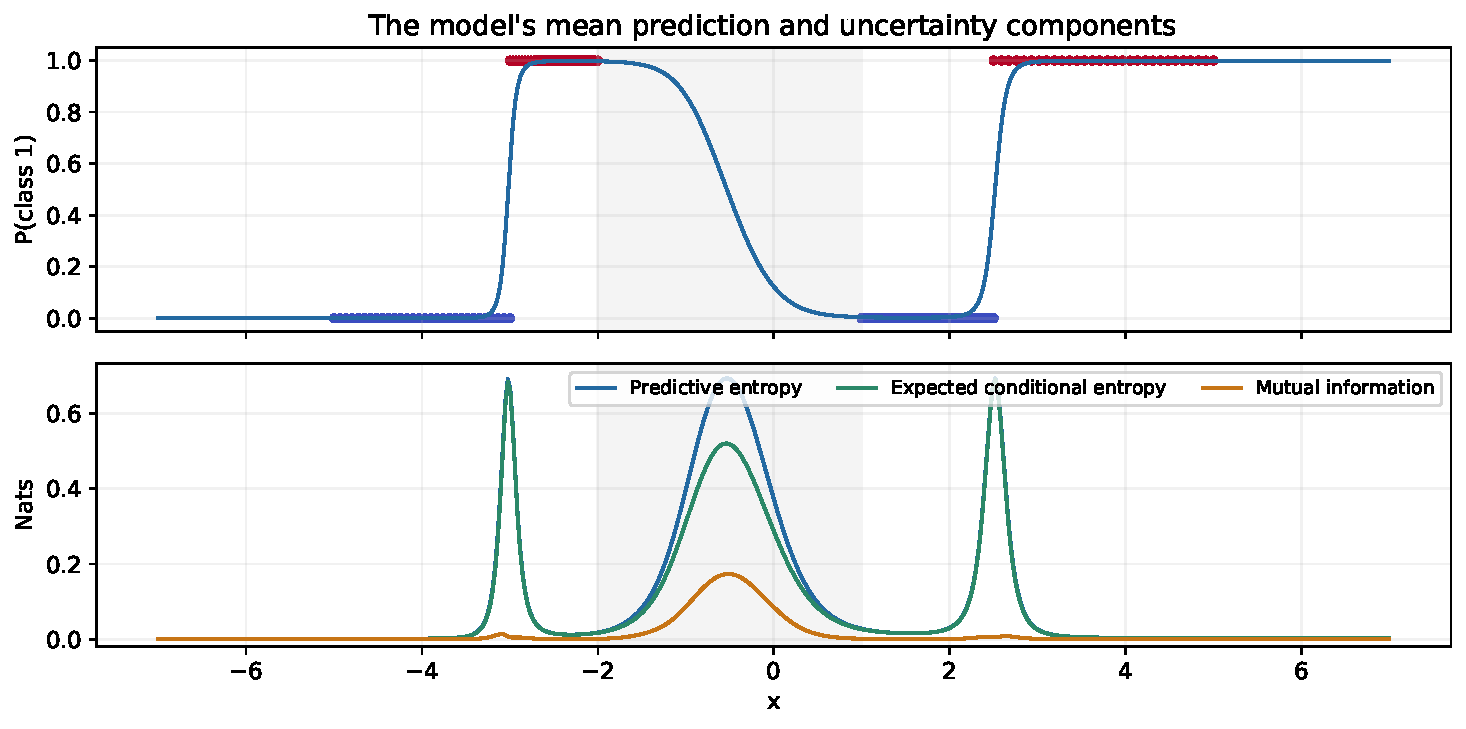
\includegraphics[width=\linewidth]{assets/toy_uncertainty.pdf}
\caption{Predictive entropy, expected conditional entropy and disagreement
for the original fitted network. The gray region has no observations;
the decomposition describes the fitted approximation, not a known label
distribution inside that region.}
\end{figure}

At $x\simeq-1.008$, the reference values are predictive entropy 0.38944,
expected conditional entropy 0.30524, and MI 0.08420 nats. At the extrapolated
point $x\simeq5.992$, MI is only $3.15\times10^{-6}$ nats. The same network
can therefore express disagreement in part of a gap and almost none in
another unsupported region. This is evidence about its approximation and
inductive behavior, rather than a general rule for detecting unfamiliar inputs.

\section{BALD: labels that distinguish current hypotheses}
\subsection{A posterior information objective}
BALD is Bayesian Active Learning by Disagreement. Houlsby et al. express a
parameter-information objective using predictive label entropies, avoiding
explicit high-dimensional posterior-entropy calculations~\cite{houlsby2011}.
For an exact Bayesian model, the desired score is
\[
 a(x)=\MI(Y;W\mid x,\mathcal D).
\]
One form is the expected information gained by updating the weight posterior:
\[
 a(x)=\E_{Y\mid x,\mathcal D}
   [\KL(p(w\mid\mathcal D,x,Y)\Vert p(w\mid\mathcal D))].
\]
When the differential entropies exist and are finite, it also equals
\[
 H(W\mid\mathcal D)
 -\E_{Y\mid x,\mathcal D}[H(W\mid\mathcal D,x,Y)].
\]
The expectation is over an as-yet unobserved label. The acquisition procedure
can evaluate the score before requesting that label.

\subsection{Derivation in the small label space}
For fixed $x$ and a weight distribution $q$, define
$\bar p_c=\int q(w)p(c\mid x,w)\dd w$. The joint distribution is
$q(w)p(c\mid x,w)$. Expanding mutual information gives
\begin{align*}
 \MI_q(Y;W\mid x)
 &=\sum_c\int q(w)p(c\mid x,w)
       \log\frac{p(c\mid x,w)}{\bar p_c}\dd w\\
 &=\E_q\left[\sum_c p(c\mid x,W)\log p(c\mid x,W)\right]
       -\sum_c\bar p_c\log\bar p_c\\
 &=H(\bar p)-\E_q[H(p(\cdot\mid x,W))].
\end{align*}
Only entropies of $C$-class label vectors are required. No entropy of a
millions-dimensional weight vector is evaluated by the code.

For the approximate distribution $q$, define its hypothetical one-label
update by
\[
 q_c(w\mid x)=\frac{q(w)p(c\mid x,w)}{\bar p_c},\qquad\bar p_c>0.
\]
The same score equals $\sum_c\bar p_c\KL(q_c\Vert q)$. This expression remains
meaningful for discrete dropout model draws, whose differential weight
entropy would not be an appropriate quantity. Retraining a restricted
network approximation after acquisition need not produce exactly this
hypothetical update. The score is a model-based decision rule, not a guarantee
that the measured uncertainty or test error will decrease after every query.

\subsection{Selecting several points is an additional approximation}
Ranking marginal BALD scores and taking the largest $k$ maximizes their sum
under a fixed-cardinality constraint. It does not generally maximize joint
information $\MI(Y_{x_1},\ldots,Y_{x_k};W\mid\mathcal D)$. Correlated or nearly
duplicate candidates may be redundant. This seminar uses the transparent
marginal-score rule and reports the acquisition batch size; it does not claim
to implement joint BatchBALD.

\section{The active-learning protocol}
\subsection{The oracle boundary and label ledger}
The acquisition code receives candidate inputs, model predictions or scores,
and a requested count. It must not inspect candidate labels. After indices
are chosen, the oracle reveals only those labels. Add the queried rows to
the labeled set and remove their indices from the pool.

Track unique indices and use random acquisition without replacement. An
unlabeled observation must not be requested twice. With $n_0$ initial labels
and acquisitions $k_1,\ldots,k_r$, the training label budget is
\[
 B_r=n_0+\sum_{j=1}^r k_j.
\]
Count the initial labels too. Limit each request by both the remaining label
budget and the pool size. Stop before requesting labels when the budget is
exhausted. Separately report any already available validation labels used for
evaluation; they are a real labeled resource even if excluded from the training
acquisition budget.

An offline dataset contains hidden labels somewhere in memory. This alone
does not invalidate an active-learning simulation. The enforceable boundary
is which functions receive or read them. Test a selector with the same inputs
and different hidden labels: acquisition indices must remain unchanged.
Labels used to audit selected class composition are inspected only after
queries, not used to choose them.


\begin{figure}[htbp]
\centering
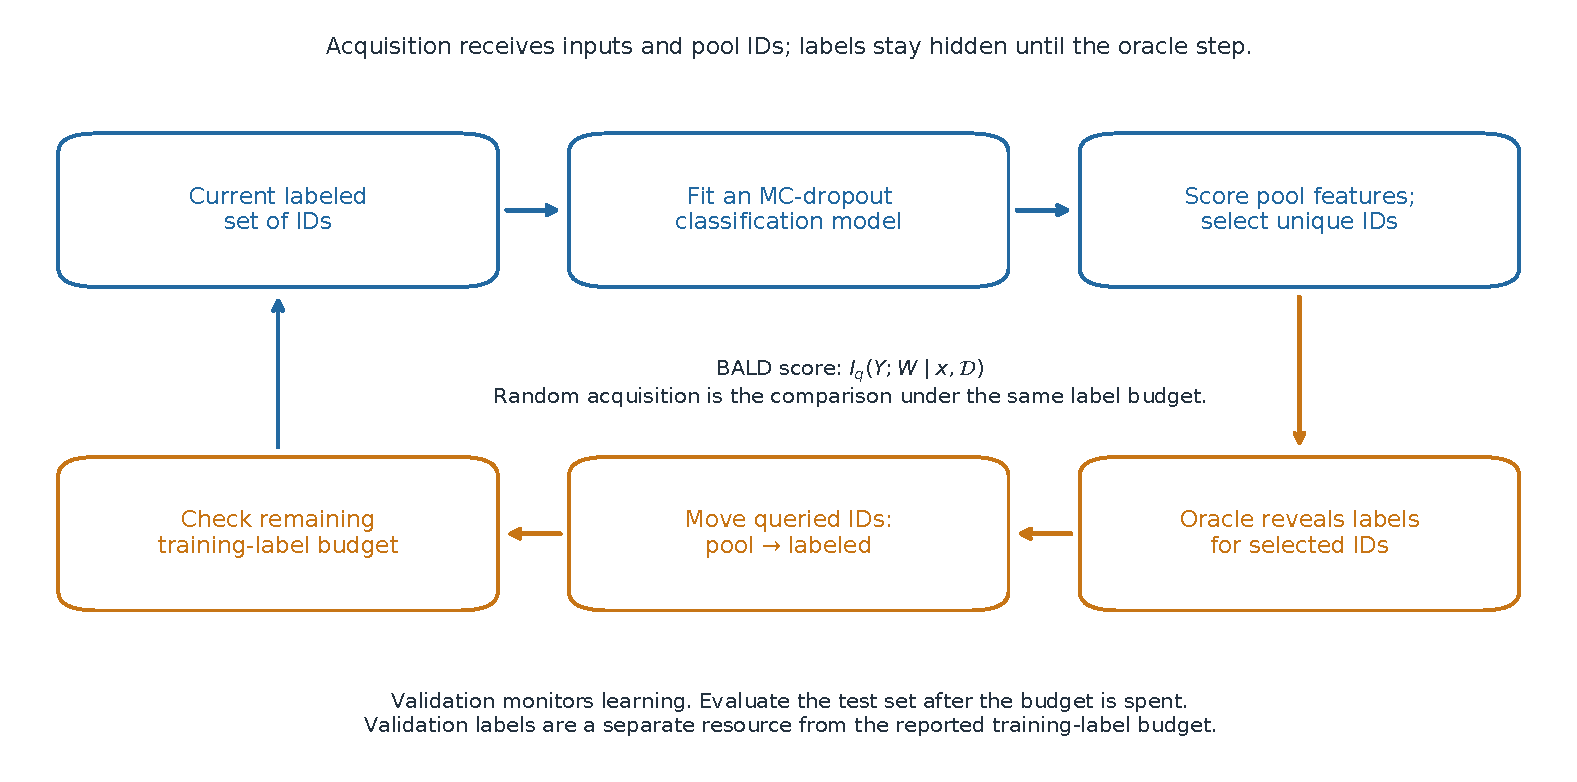
\includegraphics[width=\linewidth]{assets/active_learning_cycle.pdf}
\caption{Pool-based active learning separates input-only scoring from label
revelation. Query only after acquisition indices have been selected; move
queried points out of the pool and include their labels in the ledger.}
\end{figure}
\subsection{Keep the comparison controlled}
Within a paired replicate, use the same initial labeled indices, candidate
pool, model initialization policy, architecture, dropout probability,
optimizer schedule, training budget, and evaluation draw count for all
acquisition methods. The acquired inputs then differ by design. Use independent
random seeds across paired replicates, and preserve a record of the queried
indices and actual label counts.

State whether each round starts from the same initialization or continues
from the previous model. Either can define a useful experiment; applying
different policies to acquisition methods confounds their comparison.
A fixed number of epochs and a fixed number of optimizer updates are distinct
computational budgets when the labeled set grows. The notebook specifies one
policy and applies it equally to the methods.

Use validation data only for the announced monitoring or model-selection
purpose. Keep test data outside the acquisition and tuning loop. Record
validation curves against the number of acquired labels, not only the round
number, and evaluate the held-out test set at the planned final point.

\subsection{Read repeated results as a small controlled experiment}
Report random acquisition alongside predictive entropy and BALD when available.
Compare their accuracy and predictive negative log likelihood at equal label
budgets. A larger accuracy and a smaller NLL are preferable under those
metrics. They need not rank models identically: NLL also evaluates confidence
assigned to the observed labels.

For replicate $r$, form a paired endpoint difference, such as
$\Delta_r=\operatorname{Acc}_{\rm BALD,r}-\operatorname{Acc}_{\rm random,r}$.
Average the paired differences and report their variation. Several repeated
seeds are more informative than one winning curve, but three small trials
still do not establish a universal ranking. Variation across test images
with models fixed is different from variation across training/acquisition
runs. Avoid treating every image as an independent acquisition experiment.

\FloatBarrier
\section{Task 3: acquire pool indices without seeing labels}
\subsection{What students should do}
Complete the selector
\begin{lstlisting}
acquisition_indices(pool_ids, draws, n_query, strategy="bald", generator=None)
\end{lstlisting}
Return unique global pool IDs, not local positions in the supplied candidate
array. Strategies are random, predictive entropy, and BALD. The function has
no label argument. For score ties, prefer the smaller global ID, independent
of the order of the candidate array. A random request samples without
replacement using the supplied generator.

The contract assumes unique input IDs and valid probability draws in the
same candidate order. Reject negative requests and requests larger than the
number of candidates. A zero request returns an empty tensor of IDs. Validate
these conditions before performing any oracle update.

\subsection{Worked selection logic}
For random selection, choose local positions from a random permutation and
map them back to global IDs. For entropy or BALD, compute the corresponding
pointwise score. Sort global IDs first and then perform a stable descending
score sort. Stability preserves increasing global-ID order within equal scores.

\begin{lstlisting}
if strategy == "random":
    positions = torch.randperm(len(pool_ids), generator=generator)[:n_query]
else:
    terms = uncertainty_terms(draws)
    key = "predictive_entropy" if strategy == "entropy" else "mutual_information"
    scores = terms[key]
    by_id = torch.argsort(pool_ids, stable=True)
    ranking = torch.argsort(scores[by_id], descending=True, stable=True)
    positions = by_id[ranking[:n_query]]
selected_ids = pool_ids[positions]
\end{lstlisting}
This is the core selection step; the notebook's full implementation also
checks allowed strategy names, shapes, input uniqueness, and requested count.
The supplied \texttt{LabelOracle.query} rejects duplicate IDs, previously
queried IDs, and requests over its remaining budget atomically. A rejected
request must leave both its query history and label count unchanged.
It also rejects floating-point and Boolean IDs before conversion, avoiding
an accidental request for ID 0 when a caller passes 0.9 or False.

\subsection{The controlled one-dimensional acquisition experiment}
The 120 retained design rows become a finite pool. For each of three paired
replicates, query 12 random initial IDs without inspecting their labels.
Then make four requests of six labels. The actual budgets are
12, 18, 24, 30, and 36; all initial and new oracle requests count.

Compare random acquisition, predictive entropy, and BALD. Each budget starts
a fresh model and trains it for 1,000 full-batch steps.

The supplied small-data network has widths
\[
1\to32\to32\to2.
\]
It uses two tanh hidden layers, dropout probability 0.2 after
the first hidden layer, and input scaling $x/5$. Adam uses weight decay
$10^{-4}$ and a OneCycle schedule with maximum learning rate 0.03,
division factor 10 and final division factor 100. This smaller network
helps avoid an underfitted constant predictor on the initial 12 labels.
The original sigmoid network and its 4,000-step fit remain the motivating
example in Tasks 1 and 2.

Within a replicate
and round, methods share the initialization and training schedule; the
acquired data are allowed to differ. Evaluation uses 512 independent
mixture-of-interval samples for the displayed validation curves and 1,024
independent final test samples. Pool scoring and validation prediction use
64 model draws; final test prediction uses 256. Those evaluation labels are a separately
available resource, outside the training-label ledger.

Do not compare an acquisition curve against the fully labeled reference fit
as though both used the same number of labels. The reference fit establishes
the approximation's behavior on the original full toy design. The active
experiment studies the cost of learning from a restricted subset.

The result table includes predictive NLL and a class-summed Brier score:
\[
 \operatorname{Brier}=\frac1n\sum_{i=1}^n\sum_{c=1}^C
  (\widehat p_{ic}-\mathbf1\{y_i=c\})^2.
\]
For binary classification this convention equals twice the squared error of
the class-1 probability. State that convention when comparing numbers with
other implementations. Accuracy evaluates the chosen class, while NLL and
Brier also evaluate the full probability vector.

The executed reference comparison gives:
\begin{center}
\begin{tabular}{@{}lrrrr@{}}
\toprule
Strategy & Test accuracy & Repeat SD & Test NLL & Test Brier \\
\midrule
Random & 0.98145 & 0.00610 & 0.03840 & 0.02401 \\
Entropy & 0.83301 & 0.14208 & 1.2146 & 0.33598 \\
BALD & 0.83236 & 0.14265 & 1.1467 & 0.33570 \\
\bottomrule
\end{tabular}
\end{center}
All methods use 36 acquired labels, including the initial 12. Values average
three paired runs; the standard deviation describes repeat variation, not a
confidence interval. Last digits can differ across software stacks.

\begin{figure}[htbp]
\centering
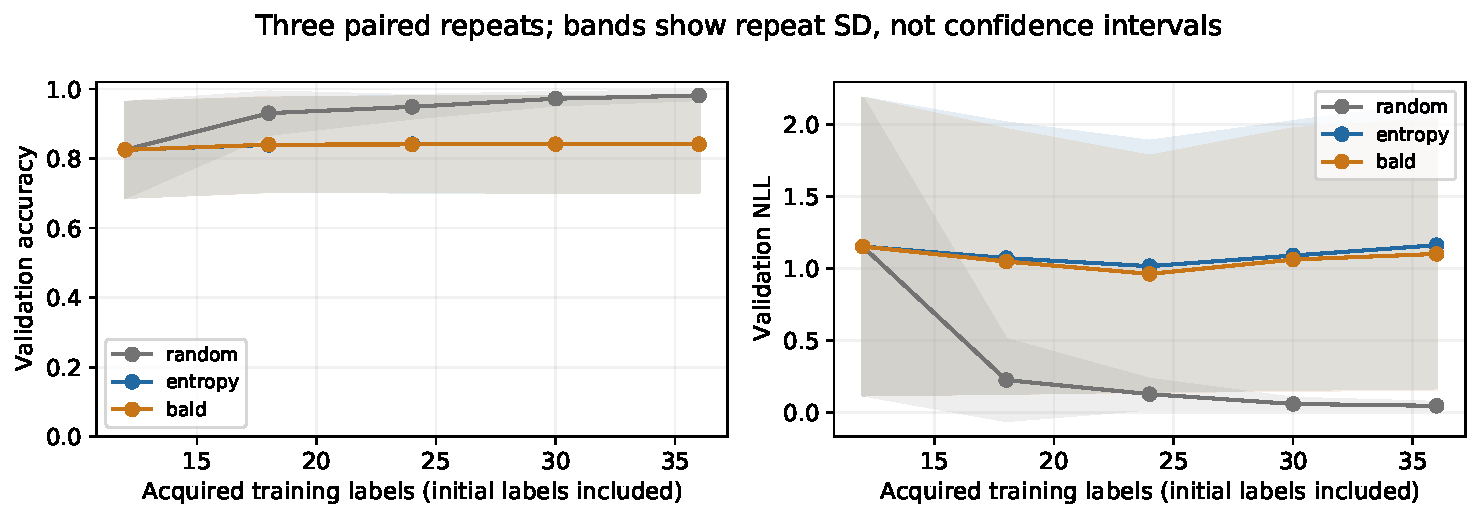
\includegraphics[width=\linewidth]{assets/toy_learning_curves.pdf}
\caption{Validation curves at common label budgets. Random acquisition
performs better in this particular toy experiment. A correct information
calculation does not guarantee an advantageous acquisition sequence under
an approximate model and a restricted batch policy.}
\end{figure}

\begin{figure}[htbp]
\centering
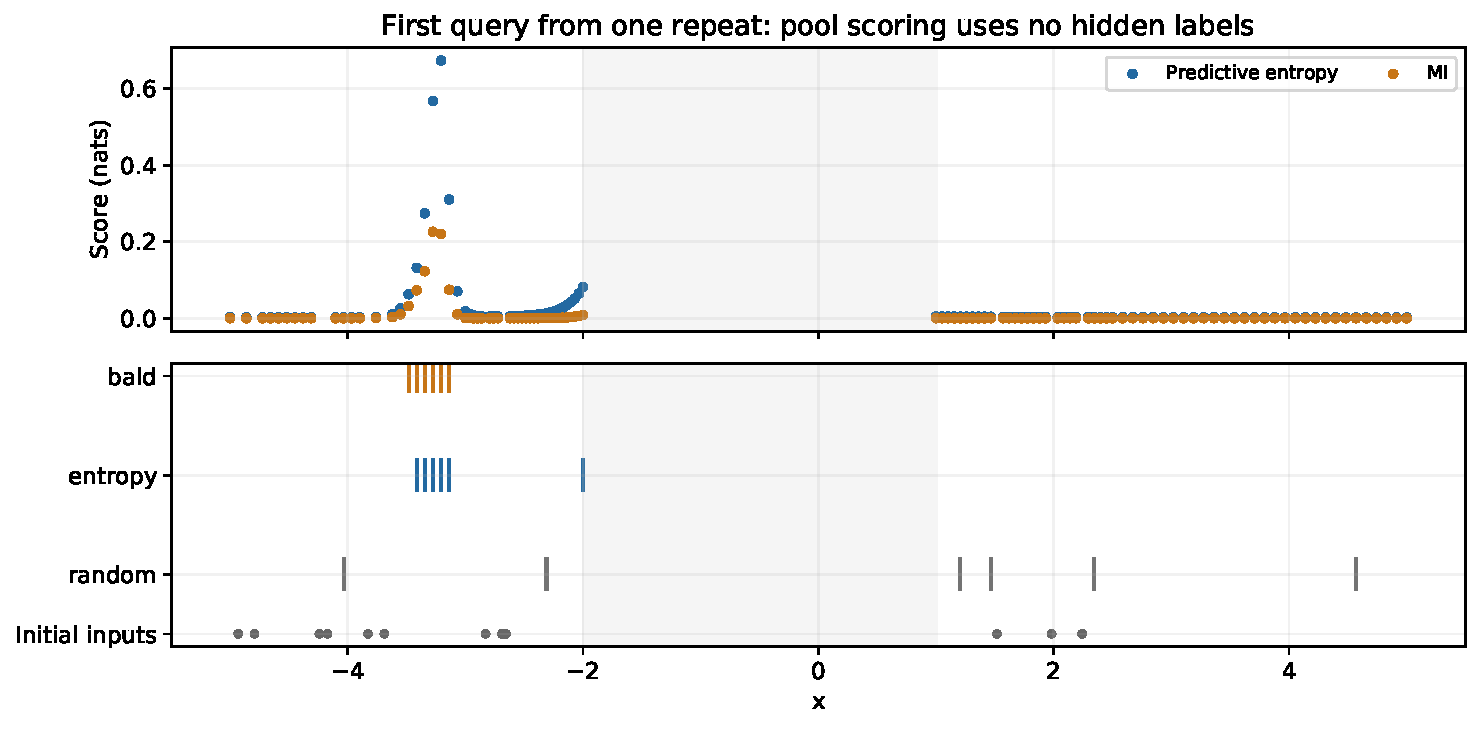
\includegraphics[width=\linewidth]{assets/toy_acquisition.pdf}
\caption{The first query in one repeat. Pointwise entropy and BALD can
spend a batch on neighboring inputs near one uncertain transition. Random
selection covers a wider part of the pool. Scores are computed before any
of the new labels are revealed.}
\end{figure}

Read this result directly: random acquisition has better mean accuracy,
NLL and Brier here. The first-query plot suggests one mechanism for failure:
pointwise ranking buys redundant neighbors, while a confidently wrong model
may assign low scores to regions that need exploration. This is not proof
that either information criterion is universally inferior. The image
experiment below gives a different comparison under a different setting.
Before discussing acquisition quality, check that a model can fit its
currently labelled observations; optimizer failure and uncertainty quality
are separate questions.

\subsection{Checks and interpretation answers}
Use handcrafted scores to check the ranking, unique IDs, exact requested
count, zero-request behavior, and stable tie order. Reordering candidate
inputs together with their probabilities must not change a deterministic
selection. Two independent random generators with the same seed should
reproduce random selection without duplicate IDs. An oracle test must verify
that failed requests consume no labels.

A correct implementation can still give a poor acquisition outcome. The
score measures model-relative information at the current fit. Approximate
training, small samples, batch redundancy, and the future evaluation
population all affect whether that information improves accuracy or NLL.
A defensible explanation cites the observed repeated-run results and the
label budget, rather than declaring BALD a universal winner.

\section{Task 4: GPU active learning for MNIST}
\subsection{Purpose and the fourth implementation}
This is a separate 45--60-minute practical. It studies a classifier that predicts
one of ten digit labels from an image; it does not fit an image density as in
the normalizing-flow practical. The same probability averaging and entropy
decomposition now operate on a multiclass CNN. The model, label oracle,
training policy, acquisition loop, and plots are supplied.

Complete the function
\begin{lstlisting}
mc_cnn_probabilities(model, images, n_draws=15, batch_size=512)
\end{lstlisting}
Inputs are uint8 images with shape $(N,1,28,28)$, on CPU or GPU. Return a CPU
float32 tensor $(T,N,10)$ with no gradient history. Preserve image order when
joining minibatches and preserve every module's original training mode.
The device comes from the model's first parameter. The supplied input helper
uses the fixed MNIST normalization $(I/255-0.1307)/0.3081$.

\subsection{Worked implementation}
\begin{lstlisting}
def mc_cnn_probabilities(model, images, n_draws=15, batch_size=512):
    if n_draws < 1 or batch_size < 1 or len(images) == 0:
        raise ValueError("Use positive draws, batch size, and nonempty images.")
    device = next(model.parameters()).device
    draws = []
    with torch.inference_mode(), mnist_dropout_only(model):
        for _ in range(n_draws):
            batches = []
            for start in range(0, len(images), batch_size):
                x = mnist_inputs(images[start:start + batch_size], device)
                batches.append(model(x).softmax(dim=-1).float().cpu())
            draws.append(torch.cat(batches, dim=0))
    return torch.stack(draws, dim=0)
\end{lstlisting}
The probability vectors are retained, rather than hard labels or averaged
logits. Taking their mean over the first axis produces the predictive
probabilities used for evaluation. Computing uncertainty requires the draws
as well as that mean.

The supplied context evaluates the model, activates only dropout modules,
and restores all individual mode flags in a finally block. Standard dropout
uses independent masks across images and across minibatches. This is valid
for each image's marginal entropy and MI. It does not give a coherent function
draw across images and does not estimate joint batch information.

\subsection{What the CPU checks establish}
A deterministic probe with known logits verifies the output values, not just
their shape. An input-sensitive pixel probe independently checks the fixed
normalization and image order across minibatches of unequal final size.
A stochastic probe verifies variation across draws and that each
class vector is finite and normalized. The probe deliberately contains batch
normalization and mixed initial module modes. Its running means and variances
must not change, and its mode flags must be restored. An interrupted
context also checks restoration after an exception.

If stochastic predictions are identical, inspect dropout activation. If
predictions differ with minibatch size even when dropout is disabled, inspect
batch-normalization mode and input order. A successful probability check does
not establish that the trained CNN is calibrated; it verifies the specified
prediction calculation.

\subsection{The supplied CNN and training policy}
The CNN uses two convolutional blocks with 16 and 32 channels, ReLU activations,
and two-by-two max pooling. A width-128 hidden layer follows the flattened
$32\times7\times7$ representation. Dropout probability 0.5 precedes the final
ten-class linear layer.

At every label budget, construct a fresh model from the prescribed seed and
train for 150 Adam updates, batch size 64, learning rate $10^{-3}$. The same
round-specific seed and policy apply to all methods in a paired replicate.
A fixed update count prevents a larger acquired dataset from silently granting
more training computation. It is a teaching budget, not a claim of optimizer
convergence at every round.

This practical uses cross entropy and stochastic dropout, without an explicitly
evaluated weight-posterior KL term. Its uncertainty scores are under the fitted
dropout approximation. Do not claim that the optimization computes an exact
posterior for a fully specified Gaussian weight prior.

\subsection{The label ledger and separate evaluation resource}
Select 6,000 candidate images uniformly from the official MNIST training set
without consulting their labels. Reserve a disjoint 1,000-image evaluation
set from the training source for learning curves. Within each paired repeat,
all methods begin with the same 100 uniformly selected initial pool IDs.
Each method queries those initial labels from its own oracle.

Four acquisitions of 100 labels produce budgets 100, 200, 300, 400, and 500.
The remaining pool shrinks as IDs are purchased, and previously acquired IDs
cannot be queried again. Random acquisition, predictive entropy, and BALD all
have the same budgets. The candidate pool and initial set are not secretly
class-balanced through hidden label inspection.

The 1,000 evaluation labels are a separate available resource and are not
charged to the acquisition-training ledger. State that cost explicitly. Their
curves do not alter the announced update count, dropout probability, stopping
budget, or acquisition method. Only after every acquisition run is finished
does the experiment evaluate the official 10,000-image test set.

Three paired replicates share initial labels and model seeds within each
replicate and use independent seeds between replicates. Entropy and BALD
choose the top 100 marginal scores; no diversity or joint-information
correction is applied. Acquisition scoring costs additional computation that
random sampling does not need. Equal training updates and label budgets do
not imply equal wall-clock cost for the methods.

\subsection{GPU setup, caching, and runtime}
The CPU checks run without CUDA. Set \texttt{RUN\_MNIST} to True to enable
the practical on a CUDA device. Otherwise the notebook prints an explicit
skip message. Install compatible PyTorch and torchvision versions and cache MNIST
before class. The default data location is shared with the preceding seminar;
results and fitted models use a separate BNN cache.

\begin{lstlisting}
BNN_MNIST_DATA   # default: /tmp/sk_bayes_mnist/data
BNN_MNIST_CACHE  # default: /tmp/sk_bayes_bnn_mnist
MNIST_RETRAIN = True
\end{lstlisting}
Set the environment variables before running the notebook to use persistent
locations. The default performs a fresh experiment; set retraining to False
only to replay a matching completed experiment. A cached replay is not a new
training measurement. Runtime depends on the GPU and software stack, so keep
executed figures available for classroom discussion.

\subsection{Accuracy, predictive NLL, and calibration measure different things}
For mean probabilities $\widehat p_i$, accuracy compares their maximum-probability
class with the observed label. Predictive NLL is
\[
 -\frac1n\sum_{i=1}^n\log\widehat p_{i,y_i}.
\]
The log is applied after averaging model probabilities. Averaging each
subnetwork's cross entropy instead evaluates expected conditional loss, which
is generally larger by Jensen's inequality and is not the same predictive
metric.

The practical also reports an expected calibration error estimate with 15
equal-width confidence bins:
\[
 \widehat{\operatorname{ECE}}
 =\sum_b\frac{n_b}{n}
  |\operatorname{accuracy}(b)-\operatorname{meanconfidence}(b)|.
\]
Empty bins contribute zero. This is a finite-sample, bin-dependent diagnostic,
not a complete calibration theorem or a proper scoring rule. Accuracy can
improve while this diagnostic worsens. Compare it with NLL and the number
of repetitions instead of treating one scalar as universal model quality.

A finite MC mean introduces numerical variation into these metrics. In
particular, $-\log\widehat p_{i,y_i}$ is generally upward biased relative to
$-\log\bar p_{i,y_i}$ at finite draw count. The experiment holds the 15-draw
budget fixed across methods. Its three repeats describe variability of the
specified training/acquisition experiment, not a broad population of all
architectures or acquisition protocols.

\subsection{Executed GPU reference}
The complete fixed-budget image experiment ran on an NVIDIA L40 in about
16 seconds in the recorded environment. This includes all 45 fits and the
final evaluations; it is not a runtime guarantee for another GPU. The full
solutions notebook, including CPU experiments and appendices, took about
80 seconds in this run.

\begin{center}
\begin{tabular}{@{}lrrrr@{}}
\toprule
Strategy & Test accuracy & Repeat SD & Test NLL & ECE \\
\midrule
Random & 0.917 & 0.003 & 0.303 & 0.057 \\
Entropy & 0.938 & 0.014 & 0.277 & 0.107 \\
BALD & 0.946 & 0.003 & 0.272 & 0.120 \\
\bottomrule
\end{tabular}
\end{center}
All methods end with 500 purchased training labels, including the initial
100. Here BALD has better average accuracy and predictive NLL than random,
while the binned ECE is worse. This contrast is worth discussing: correct
class decisions, good predictive log probabilities, and agreement of confidence
with empirical correctness are distinct criteria. These three repeats do
not support a universal ordering of acquisition strategies.

\begin{figure}[htbp]
\centering
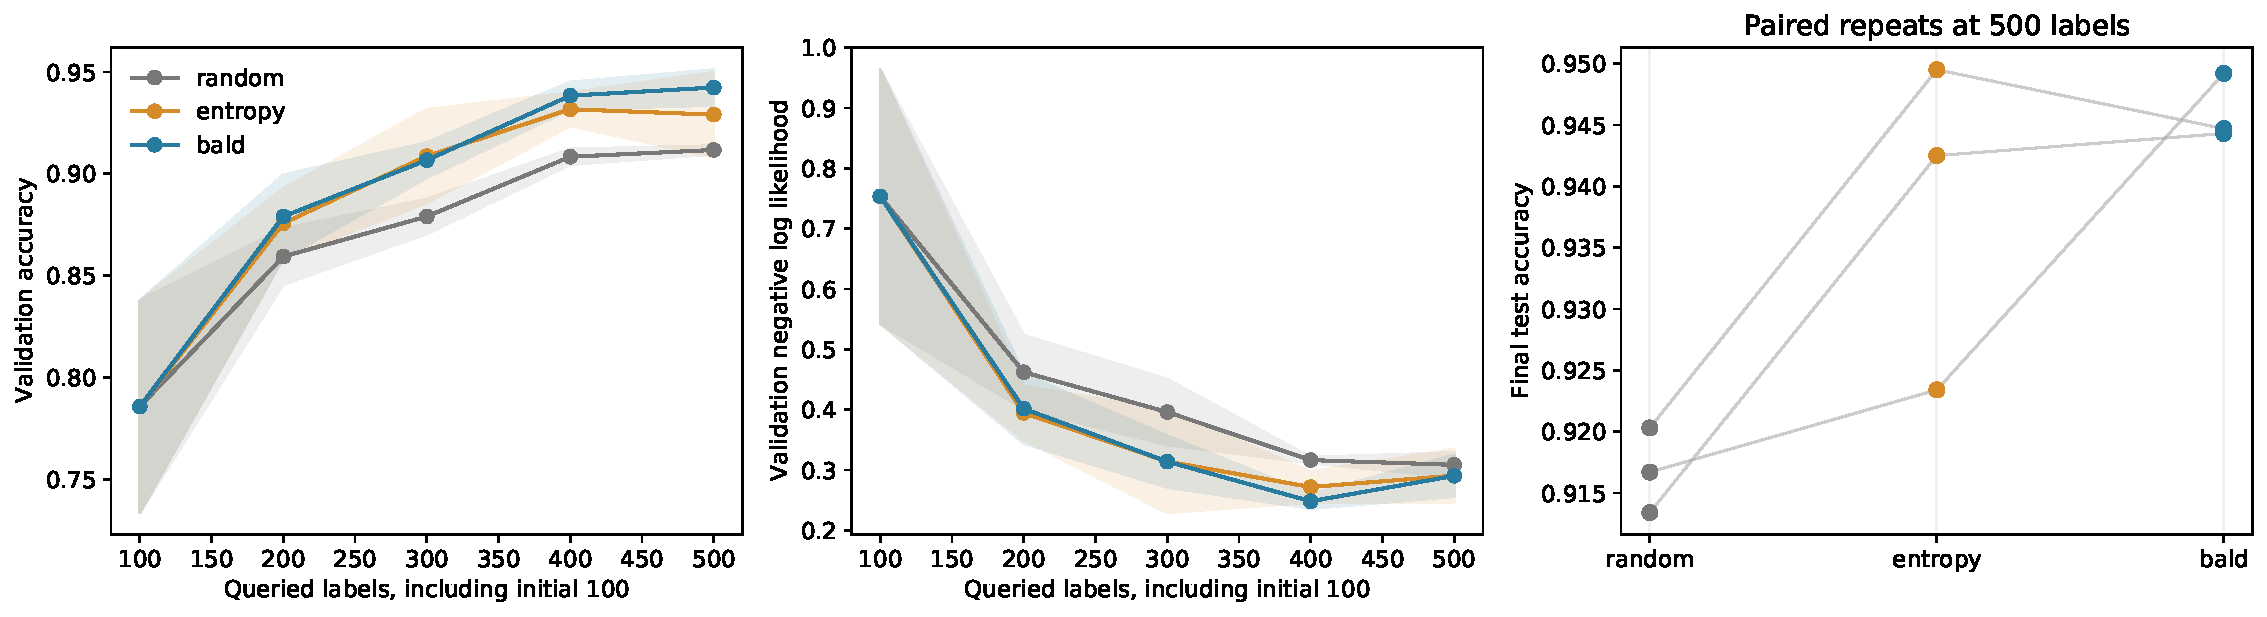
\includegraphics[width=\linewidth]{assets/mnist_learning_curves.pdf}
\caption{The GPU practical's learning curves and paired final-test outcomes.
Common initial labels and model seeds make the endpoint comparisons paired.
Bands show repeat standard deviation, rather than a confidence interval.}
\end{figure}

\subsection{Read the figures without using future labels}
Learning curves show accuracy and NLL against the actual number of purchased
labels. Shaded bands are one standard deviation across the three repeats,
not confidence intervals. Connected test endpoints show the pairing between
methods that began with the same data and model seed.

At the first acquisition, entropy and BALD start from the same fitted CNN.
A scatterplot of predictive entropy against MI, colored by expected conditional
entropy, shows how the criteria can differ before any new labels are known.
Highlighting the selected BALD batch does not require its labels.

The acquisition image panels display the first eight selected digits for each
strategy in the first repeat. Their labels are revealed after selection and
then shown as captions. Several similar selected digits can expose the
redundancy of marginal batch ranking. A class-count heatmap audits labels
already bought; it never examines the remaining hidden pool labels.
Class balance is a useful diagnostic, not the objective of either information
criterion.

\begin{figure}[htbp]
\centering
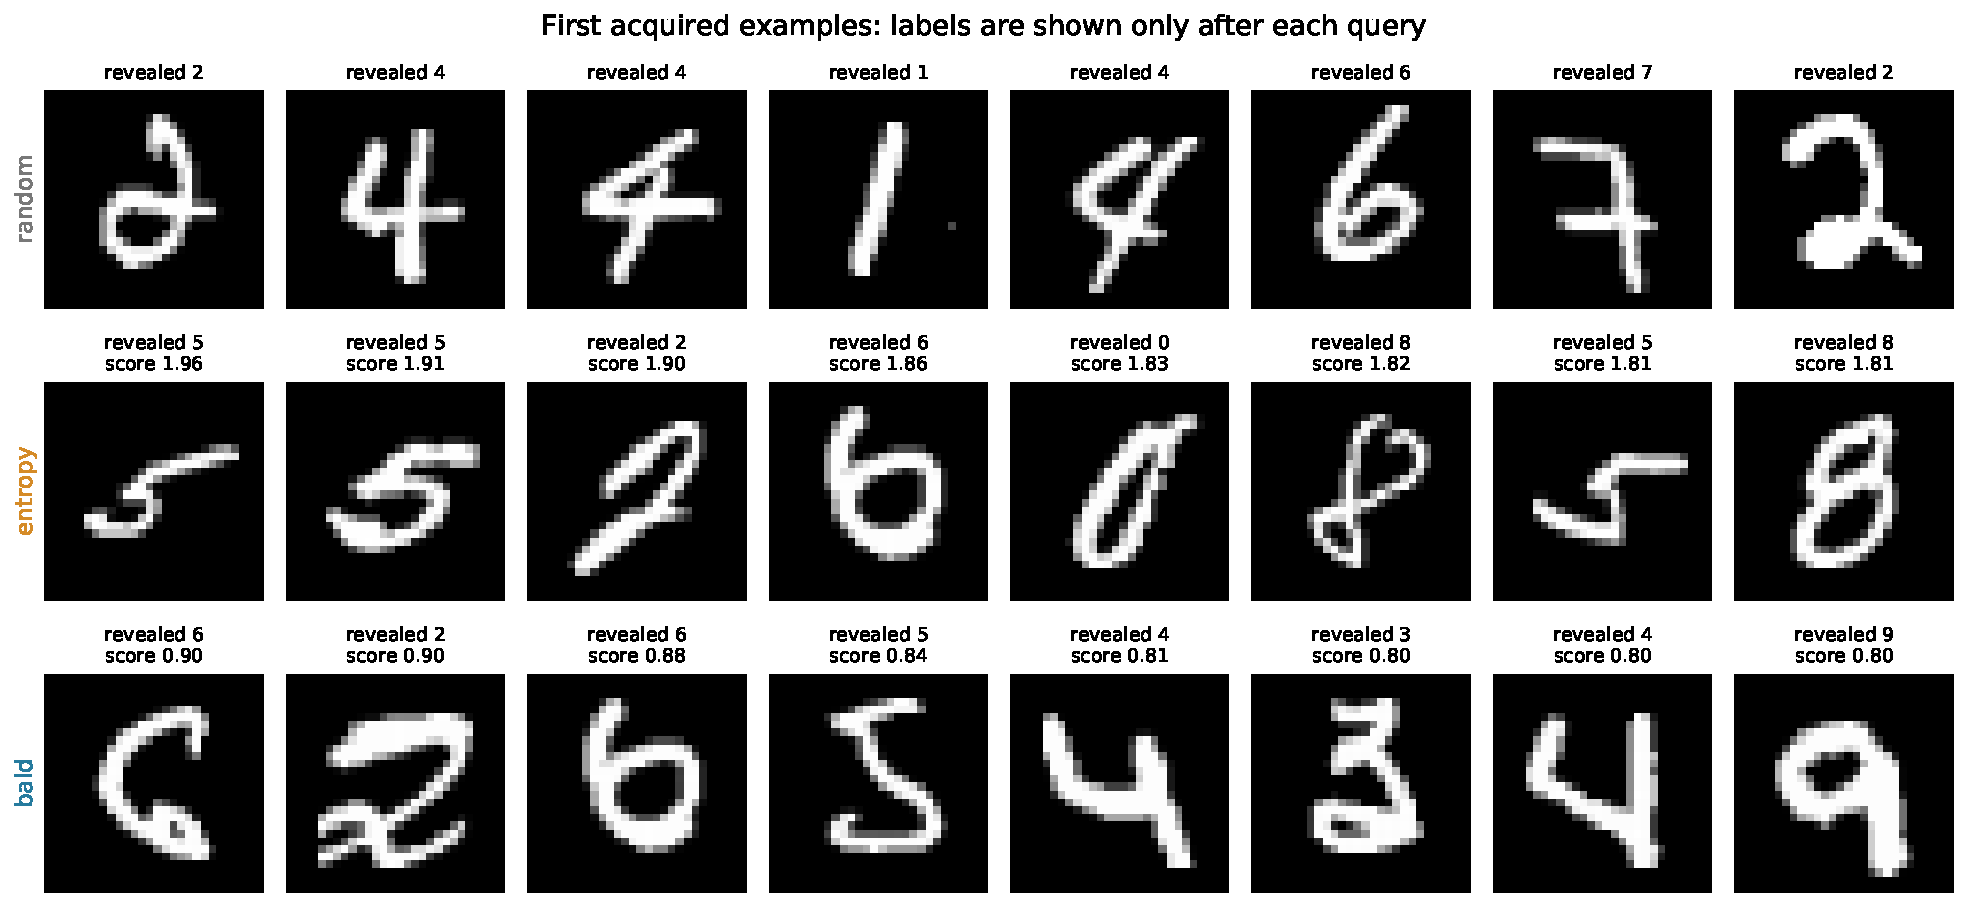
\includegraphics[width=\linewidth]{assets/mnist_acquired_digits.pdf}
\caption{First selected MNIST examples in the first repeat. Labels appear
only after they have been purchased. Entropy and BALD may choose different
images from the same starting model because their scores measure different
properties of its predictive mixture.}
\end{figure}

\subsection{Worked interpretation and questions}
A suitable explanation identifies the common budget and model policy before
comparing outcomes. It describes whether a ranking persists across paired
repeats and whether the observed difference is large relative to their spread.
It also separates classification accuracy from confidence quality.

Ask why two criteria select different digits from the same starting CNN,
why repeated similar digits can all rank highly, and which resources a
label-budget plot omits. Require students to account for evaluation labels
and acquisition computation. A planned follow-up can study different batch
selection or distribution shift, but the existing test set would then be a
development resource if its results influence that choice.

\appendix
\section{Data geometry, intrinsic ambiguity, and unsupported inputs}
This optional appendix reuses the supplied toy fit and uncertainty calculations;
it adds no implementation task. Enable the appendix experiments only after
completing the core tasks.

For overlapping intervals, use class 0 on $[-2,2]$ and class 1 on $[0,4]$.
For a separate population that chooses either interval with equal probability
and samples uniformly inside it, the conditional class-1 probability is
$1/2$ in $(0,2)$. The two intervals have equal lengths, so their population
densities agree there. Outside their overlap but inside the union, only one
class has positive density.

The overlap has probability mass $1/2$ under this population. Therefore its
Bayes classification error is $1/4$, and the population-average conditional
label entropy is $(\log2)/2$. These are references for the specified population,
not identities that a finite trained dropout network must reproduce exactly.
Expected conditional entropy can approach the label ambiguity when the model
and approximation fit well; underfitting can also increase that entropy.

For separated intervals, use class 0 on $[-5,-3]$ and class 1 on $[3,5]$.
The reference population has no support in $(-3,3)$. It does not specify a
unique ground-truth label probability in the gap. Inspect the model's
extrapolation and disagreement without interpreting either as a known
conditional probability of that population. A high-disagreement gap is a
possible result of the approximation, not a theorem about dropout.

Changing the dropout rate requires refitting. Increasing it can change
regularization, optimization, fit, and the approximation family at once.
Do not interpret a wider probability band by itself as evidence that the
posterior approximation improved.

\section{Monte Carlo budgets and redundant acquisition batches}
This optional material separates integration precision from statistical
information. Compare repeated MC summaries of one fixed fitted model at
several draw counts. Expect less integration variability as the count grows,
while allowing individual entropy and MI estimates to fluctuate. Their
finite-sample nonlinear bias is another reason not to equate a small estimate
with the absence of model disagreement.

The draw count and acquisition batch size are different budgets. More draws
can improve a pointwise ranking; requesting more top-ranked points can buy
redundant labels. For example, several near-identical inputs may all disagree
with the model in the same way. Summing marginal information counts that
shared distinction repeatedly, whereas joint information considers what
additional labels contribute after the first one.
The BatchBALD method explicitly addresses joint label information~\cite{batchbald}.
Its calculation would require coherent model draws across candidate inputs;
the ordinary dropout rows in the image practical are only pointwise marginal
samples and should not be reused as if they represented a joint function draw.

The core and image practical both use pointwise ranking. They are deliberately
transparent about that limitation. A planned extension could study diverse
batches or a joint-information approximation, with its own compute budget
and repeated comparison against random acquisition. The current test results
must not be reused to select such an extension and then reported as its final
independent evaluation.

Teaching-material provenance. The original BNN active-learning notebook supplied
in this directory credits Ivan Nazarov. The one-dimensional construction is
retained from cells 0--9 of the supplied 2025 uncertainty seminar. The new
notebooks implement the displayed methods locally and keep both reference
notebooks unchanged.

\begin{thebibliography}{9}
\bibitem{gal2016}
Yarin Gal and Zoubin Ghahramani.
\emph{Dropout as a Bayesian approximation: representing model uncertainty in
deep learning}. ICML, 2016.
\href{https://proceedings.mlr.press/v48/gal16.html}{PMLR 48:1050--1059}.

\bibitem{houlsby2011}
Neil Houlsby, Ferenc Husz\'ar, Zoubin Ghahramani, and M\'at\'e Lengyel.
\emph{Bayesian active learning for classification and preference learning}.
2011. \href{https://arxiv.org/abs/1112.5745}{arXiv:1112.5745}.

\bibitem{gal2017}
Yarin Gal, Riashat Islam, and Zoubin Ghahramani.
\emph{Deep Bayesian active learning with image data}. ICML, 2017.
\href{https://proceedings.mlr.press/v70/gal17a.html}{PMLR 70:1183--1192}.

\bibitem{batchbald}
Andreas Kirsch, Joost van Amersfoort, and Yarin Gal.
\emph{BatchBALD: efficient and diverse batch acquisition for deep Bayesian
active learning}. NeurIPS, 2019.
\href{https://proceedings.neurips.cc/paper/2019/hash/95323660ed2124450caaac2c46b5ed90-Abstract.html}{Paper}.
\end{thebibliography}
\end{document}
